\documentclass[11pt,a4paper]{article}
\usepackage[margin=2.5cm]{geometry}
\usepackage{amsmath,amssymb,amsthm}
\usepackage{booktabs}
\usepackage{graphicx}
\usepackage{xcolor}
\usepackage{tikz}
\usetikzlibrary{arrows.meta,positioning}
\usepackage[hidelinks]{hyperref}

\newtheorem{proposition}{Proposition}
\newtheorem{definition}{Definition}
\theoremstyle{remark}
\newtheorem{remark}{Remark}
\newtheorem{example}{Example}

\title{Bilinear Realisations of Truncated Chen--Fliess Series\\ and Path Signatures: a Tutorial}
\author{Gary Green\\University of York}
\date{}

\begin{document}
\maketitle

\begin{abstract}
This tutorial shows how to turn a truncated Chen--Fliess series, or a truncated path signature, into a small bilinear state-space model, and how to fit such a series to sampled data.
It covers systems with a letter for time (a drift) and systems without one, where the series is a path signature.
The methods are standard: iterated integrals, the Hankel matrix indexed by words, minimal and graded realisations, Volterra kernels and the Lie--Hankel matrix built from Lyndon words.
The tutorial works through them on a synthetic example and four test systems, with code that reproduces every number, and states the practical lessons learnt in applying them: how to compute the iterated integrals from formulas and from samples, how to set up the Hankel matrix of a truncated series, why each window needs its own starting value, what the fitted coefficients can and cannot tell, why the sizes of realisations of fitted series must be compared with their largest possible values, and how far a realisation can be trusted beyond the window it was fitted on.
\end{abstract}

\section{Introduction}
Many systems are studied through the way a measured output responds to an input, rather than through known equations.
For a linear system, one function describes this response: the impulse response.
For a nonlinear system, Volterra replaced it by a hierarchy of kernels, one for each order of interaction between inputs at different times \cite{Volterra1930}; Brockett connected these kernels to the geometry of the system \cite{Brockett1976}.
The kernels are functions of many time arguments.
They are hard to estimate from data, and they do not by themselves give a model with a finite state \cite{WrayGreen1994}.

Fliess reorganised the same information \cite{Fliess1981}, building on Chen's iterated integrals \cite{Chen1957}.
The Chen--Fliess series attaches one number to each word: a finite sequence drawn from an alphabet with one letter for the passage of time and one letter for each input.
When there is no letter for time, the iterated integrals are the path signature of the inputs, now used widely for time series \cite{Lyons1998,FrizVictoir2010,ChevyrevKormilitzin2016}.

The series has a realisation theory that mirrors linear systems theory.
A linear impulse response can be reproduced by a finite linear state-space model, found from its Hankel matrix by the Ho--Kalman method \cite{Kalman1963,HoKalman1966}.
In the same way, a Chen--Fliess series can be reproduced by a finite bilinear model, found from a Hankel matrix indexed by words \cite{Fliess1974,Schutzenberger1961,Isidori1973,DAlessandroIsidoriRuberti1974}.
Hespel and Jacob developed this into numerical methods \cite{HespelJacob1991,HespelJacob1998}.
The link between finite series and nilpotent structure is old.
Crouch showed that a finite Volterra series, polynomial in the input, has a realisation whose Lie algebra is nilpotent \cite{Crouch1981}; that condition concerns brackets of the vector fields, not products of matrices.
Sontag studied polynomial response maps \cite{Sontag1979}, and Krener the approximation of nonlinear systems by bilinear ones to a given order \cite{Krener1975}.
Shaikin used nilpotency of the Lie algebra of the input matrices, with the drift excluded, to obtain finite filters for stochastic bilinear systems \cite{Shaikin2004}.

In practice only a truncated part of the series is known, estimated up to some word length $K$ from a finite record of data.
This tutorial collects, in one place and with code, what is needed to realise such a series and to fit it.
Section~\ref{sec:background} introduces words, iterated integrals and the series, and how to compute the integrals.
Section~\ref{sec:realisation} introduces bilinear realisations, the Hankel matrix of a truncated series, and two ways of building a realisation.
Section~\ref{sec:validation} works through four systems with exact coefficients: the driven Duffing oscillator, a Duffing-like system without a letter for time, the Heisenberg integrator, whose series is finite, and a system with four input channels.
Section~\ref{sec:regression} fits truncated series to sampled data, Section~\ref{sec:kernels} derives Volterra kernels from the coefficients, and Section~\ref{sec:lyndon} introduces Lyndon words and the Lie--Hankel matrix.
Section~\ref{sec:lessons} lists the practical lessons.

\section{Background}\label{sec:background}
\subsection{Letters, words and iterated integrals}
Consider a system with state $x$, input $u(t)$ and output $y$,
\begin{equation}\label{eq:system}
\dot x=f_0(x)+\sum_{i=1}^m f_i(x)\,u_i(t),\qquad y=h(x),\qquad x(0)=x_0 .
\end{equation}
The vector field $f_0$ moves the state when there is no input; it is the drift.
Each $f_i$ is the direction in which input $i$ pushes the state.

The alphabet has one letter for each of these.
Letter $0$ stands for the drift, and letters $1,\dots,m$ for the inputs.
A word is a finite sequence of letters, $w=(a_1,\dots,a_L)$, read in time order: $a_1$ acts first.
Its length is $|w|=L$, and $()$ is the empty word.
To each word belongs an iterated integral,
\begin{equation}\label{eq:iterated}
I_{()}(t)=1,\qquad I_{(a_1,\dots,a_L)}(t)=\int_0^t I_{(a_1,\dots,a_{L-1})}(s)\,u_{a_L}(s)\,ds,\qquad u_0\equiv 1 .
\end{equation}
Each letter integrates the previous integral against its own signal: the drift letter against time, an input letter against that input.

\begin{example}[The first iterated integrals, one input]\label{ex:integrals}
With one input ($m=1$), the integrals of the words of length 1 and 2 are
\begin{align*}
I_{(0)}(t)&=t, & I_{(1)}(t)&=\int_0^t u(s)\,ds,\\
I_{(0,0)}(t)&=\tfrac{t^2}{2}, & I_{(0,1)}(t)&=\int_0^t s\,u(s)\,ds,\\
I_{(1,0)}(t)&=\int_0^t (t-s)\,u(s)\,ds, & I_{(1,1)}(t)&=\tfrac12\Bigl(\int_0^t u(s)\,ds\Bigr)^2 .
\end{align*}
A word of drift letters alone is a power of time.
The words $(0,1)$ and $(1,0)$ contain the same letters in a different order, and their integrals weight the input differently: early input counts most in $I_{(1,0)}$, late input in $I_{(0,1)}$.
\end{example}

The integral of a word of length $L$ is scaled by $t^L/L!$.
Over a short window the integrals of long words are therefore very small.
This matters for fitting (Section~\ref{sec:regression}).

When the system has no drift, $f_0=0$, there is no letter for time.
The letters are the input channels alone, and the iterated integrals are the signature of the path $\xi(t)=\int_0^tu(s)\,ds$ \cite{Chen1957,Lyons1998}.
With two channels, for example, $I_{(1,2)}(t)=\int_0^t\xi_1(s)\,u_2(s)\,ds$.
The state then moves only when the path moves: with no input, nothing changes.
Without a drift the integral of a word of length $L$ is scaled by $(Ut)^L/L!$, where $U$ is the size of the inputs, because every letter integrates against an input.
The rest of this section, and the realisation theory that follows, apply unchanged; only the alphabet differs.

\subsection{Computing the iterated integrals}\label{sec:computing}
The integrals are computed in one of two ways, according to what is known about the input.
When the input is known as a formula, they are the solution of the linear equations $\dot I_{wa}=u_aI_w$ (with $u_0=1$ for the drift letter), integrated by the eighth-order Dormand--Prince method \cite{HairerNorsettWanner1993} with the input evaluated exactly.
Each integral is integrated in units of its own scale, so that the tolerance of the integrator is a relative one even for the tiny integrals of long words.
For words of input letters alone and of drift letters alone, which have closed forms, the largest relative error up to length 8 is <<acc_closed>>.
When the input is known only as samples, as with recorded data and in every fit of Section~\ref{sec:regression}, the integrals are computed by the iisignature library \cite{ReizensteinGraham2020} on the sampled path: $(t,\int_0^tu)$ with a letter for time, $\int_0^tu$ without.
The integral of $u$ at the samples is taken as the exact integral of a cubic spline through the samples of $u$, and iisignature gives the exact iterated integrals of the path that joins those points by straight lines.
Its difference from the exact integrals is of second order in the sampling step.
For the input $u(t)=0.3\sin 6\pi t+0.1\sin 14\pi t$, sampled every 1\,ms over 0.15\,s, the largest difference at the end of the window, relative to the largest integral of the same length, is <<iis_1ms>> up to length 6, and <<iis_01ms>> at a step of 0.1\,ms.
For the faster inputs of Section~\ref{sec:regression} the error of each integral, relative to its own size over the window, is up to <<colerr_2>> at length 2 and <<colerr_6>> at length 6.

\subsection{The Chen--Fliess series}
The output of \eqref{eq:system} is
\begin{equation}\label{eq:cfs}
y(t)=\sum_{w} c_w\,I_w(t),\qquad c_{(a_1,\dots,a_L)}=\bigl(L_{f_{a_1}}L_{f_{a_2}}\cdots L_{f_{a_L}}h\bigr)(x_0),
\end{equation}
summed over all words \cite{Fliess1981,Isidori1995}; without a drift the same formula holds with the channel letters alone.
Here $L_fg=\nabla g\cdot f$ is the rate of change of $g$ along $f$, the Lie derivative.
The coefficient of a word measures how strongly that sequence of actions changes the output, starting from $x_0$.
It is a single number for each word.
The coefficients depend on the initial state $x_0$ but not on the input.

The empty word has $I_{()}=1$, so its coefficient $c_{()}=h(x_0)=y(0)$ is a constant: the output at the start of the window.
Each window of data is therefore shifted to start at zero before it is fitted, and the series is fitted to $y(t)-y(0)$, with $c_{()}=0$.
The model then predicts $y(t)-y(0)$, and adding the first sample of the window, $y(0)$, gives $y(t)$.
This is done separately for every window, because each window starts from its own state $x_0$ and so has its own $y(0)$.
The realisations below are built for the shifted series in the same way.
Placing $y(0)$ in the empty-word coefficient instead gives realisations of the same size for the driven Duffing series, at every order in Table~\ref{tab:dims}.

The truncated series of order $K$ keeps the words up to length $K$ and sets every longer coefficient to zero.
It approximates the output over a short enough window.

\section{Bilinear realisations of a truncated series}\label{sec:realisation}
\subsection{Bilinear realisations}
A bilinear system has a state that evolves linearly at each instant, with matrices that depend on the input:
\begin{equation}\label{eq:bilinear}
\dot z=A_0z+\sum_{i=1}^mu_i(t)\,A_iz,\qquad \hat y=\mu^\top z,\qquad z(0)=\lambda .
\end{equation}
Its output also has a Chen--Fliess series, and its coefficients are products of its matrices:
\begin{equation}\label{eq:realisation}
c_w=\mu^\top A_{a_L}\cdots A_{a_1}\lambda\qquad\text{for } w=(a_1,\dots,a_L).
\end{equation}
Reading a word letter by letter moves the state, $z\mapsto A_az$, and the read-out $\mu$ turns the final state into a number.
A realisation of a set of coefficients is a choice of $(\lambda,\{A_a\},\mu)$ that reproduces every coefficient through \eqref{eq:realisation}.
A realisation is a finite model.
It can be integrated as an ordinary differential equation for any new input, and its kernels follow from its matrices.

A realisation is reachable if the states $A_{a_L}\cdots A_{a_1}\lambda$, over all words, span the whole state space.
It is observable if the read-outs $\mu^\top A_{a_L}\cdots A_{a_1}$ span the whole dual space.
It is minimal if no realisation with fewer states reproduces the same coefficients.
As in the linear case, a realisation is minimal if and only if it is reachable and observable, and two minimal realisations differ only by a change of basis \cite{DAlessandroIsidoriRuberti1974,BerstelReutenauer2011}.

\subsection{The Hankel matrix}
The Hankel matrix of a set of coefficients has one row and one column for each word.
The entry in row $u$ and column $v$ is the coefficient of the word $uv$, $u$ followed by $v$:
\begin{equation}
H[u,v]=c_{uv}.
\end{equation}
For a realisation, $c_{uv}=(\mu^\top A_v)(A_u\lambda)$, where $A_u$ is the product along $u$.
So $H$ is a product of a matrix with $n$ columns and a matrix with $n$ rows, and its rank is at most $n$.
Fliess showed that the rank of the Hankel matrix is exactly the size of a minimal realisation \cite{Fliess1974}.
A factorisation $H=PQ$ of rank $r$ gives one.
With $H_a[u,v]=c_{uav}$, the matrices are $A_a=(P^+H_aQ^+)^\top$, the initial state is the row of $P$ for the empty word, and the read-out is the column of $Q$ for the empty word.

For a series truncated at order $K$, the staircase Hankel matrix is defined as follows: the rows and columns are all words of length $0$ to $K$, and
\begin{equation}
H[u,v]=\begin{cases} c_{uv}, & |u|+|v|\le K,\\ 0, & |u|+|v|>K.\end{cases}
\end{equation}
The zeros are not a choice; they are the coefficients of the truncated series beyond order $K$.
A row word of length $\ell$ has non-zero entries only in columns of length at most $K-\ell$, so the non-zero entries form a staircase.
The same holds for every $H_a$.
Every entry of $H$ and of every $H_a$ is therefore known: either a coefficient up to order $K$, or a zero.

\begin{example}[The staircase Hankel matrix at $K=2$]\label{ex:hankel}
For the Duffing oscillator of Section~\ref{sec:validation}, truncated at $K=2$, the non-zero coefficients are
<<ex_coefs>>.
The words up to length 2 are $()$, $(0)$, $(1)$, $(0,0)$, $(0,1)$, $(1,0)$, $(1,1)$, and the staircase Hankel matrix is
\[
<<ex_hankel>>
\]
Its rank is <<ex_rank>>, so the truncated series has a minimal realisation with <<ex_rank>> states.
\end{example}

\subsection{Truncation and nilpotency}
\begin{definition}
A realisation is \emph{nilpotent of index $K+1$} if $A_{a_{K+1}}\cdots A_{a_1}=0$ for every choice of $K+1$ letters. (Shorter products may also vanish; the index here is the length named, not necessarily the smallest one.)
\end{definition}
A nilpotent realisation reads any word longer than $K$ to zero.
Its coefficients beyond order $K$ are therefore zero, as those of a truncated series are.

\begin{proposition}\label{prop:minimal}
A minimal realisation of a series truncated at order $K$ is nilpotent of index $K+1$.
\end{proposition}
\begin{proof}
Let $w$ be a word of length $K+1$.
For all words $u$ and $v$, $\mu^\top A_vA_wA_u\lambda=c_{uwv}=0$, because $|uwv|>K$.
Since the realisation is reachable, the vectors $A_u\lambda$ span the state space, so $\mu^\top A_vA_w=0$ for every $v$.
Since it is observable, the vectors $A_v^\top\mu$ span the state space, so $A_w=0$.
\end{proof}

\begin{remark}
A realisation that is not minimal can reproduce a truncated series without being nilpotent, if it contains states that the input cannot reach or the output cannot see.
Its coefficients beyond order $K$ are still zero, so its output still contains no terms beyond order $K$.
Nilpotency is therefore sufficient for a realisation to have no terms beyond order $K$, but not necessary; it is guaranteed for minimal realisations.
For a reduced realisation, which reproduces the series only approximately, nilpotency is the simple way to guarantee that no terms beyond order $K$ appear.
\end{remark}

\begin{remark}[Validity]
The solution of \eqref{eq:bilinear} can be written as a sum over words of products of the matrices times iterated integrals, obtained by substituting the equation into itself repeatedly (the Peano--Baker series); its coefficients are given by \eqref{eq:realisation}.
In a nilpotent realisation every product of more than $K$ matrices is zero, so this sum stops at length $K$, and the output is exactly the truncated series $\sum_{|w|\le K}c_wI_w(t)$, for all times and all inputs.
The integrals of drift words are powers of time, $I_{(0,\dots,0)}(t)=t^L/L!$, and the others are integrals of the input weighted by powers of time.
Such an output need not blow up; for example, it stays bounded if every coefficient involving the drift letter vanishes and the iterated integrals of the inputs stay bounded.
But its drift words are polynomials in time, which cannot decay, so outside the window it is in general a poor description of the system.
It is also true that every matrix of a nilpotent realisation, and every combination $A_0+\sum_iu_iA_i$, has all its eigenvalues equal to zero.
That is a consequence of nilpotency, not a test for it: matrices that each have only zero eigenvalues can have products that never vanish.
Nor are computed eigenvalues a reliable sign of nilpotency: a perturbation of size $\varepsilon$ of a nilpotent $n\times n$ matrix can move its eigenvalues by as much as $\varepsilon^{1/n}$, so the products themselves must be checked.
A nilpotent realisation describes the system only over the window on which the truncated series does; Section~\ref{sec:forward} shows how this window ends in one example.
\end{remark}

\subsection{The staircase realisation}\label{sec:construction}
The staircase Hankel matrix is factorised by a singular value decomposition, $H=U\Sigma V^\top$.
This writes $H$ as a sum of simple rank-one pieces, ordered by their sizes $\sigma_1\ge\sigma_2\ge\dots$, the singular values.
The rank $r$ is the number of singular values above $\tau\sigma_1$, for a relative tolerance $\tau$; discarding the small pieces gives a smaller model of a nearby series.
With $P=U_r\Sigma_r^{1/2}$ and $Q=\Sigma_r^{1/2}V_r^\top$, the realisation follows from the formulas of the previous section.
When no non-zero singular value is discarded, this is a minimal realisation, and by Proposition~\ref{prop:minimal} it is nilpotent.
When singular values are discarded to obtain a smaller model, the result is a realisation of a nearby series of lower rank.
That series is in general not truncated, and the realisation is no longer nilpotent.

\subsection{The graded construction}
The graded construction keeps the structure of the word-length grading at every step.
Its state is divided into blocks, one for each word length $\ell=0,\dots,K$.
Every matrix $A_a$ moves the state from block $\ell$ to block $\ell+1$ only (Figure~\ref{fig:grades}).
After $K+1$ letters there is no block left, and the state is zero.

\begin{figure}[t]\centering
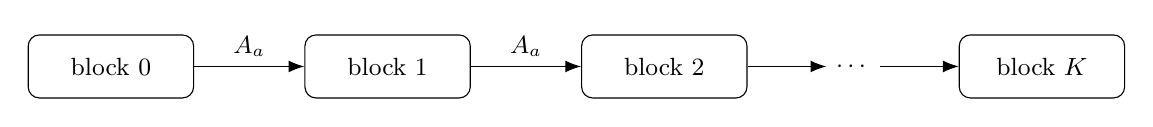
\begin{tikzpicture}[node distance=1.4cm, every node/.style={font=\small}]
\node[draw, rounded corners, minimum width=2.1cm, minimum height=0.8cm] (g0) {block 0};
\node[draw, rounded corners, minimum width=2.1cm, minimum height=0.8cm, right=1.4cm of g0] (g1) {block 1};
\node[draw, rounded corners, minimum width=2.1cm, minimum height=0.8cm, right=1.4cm of g1] (g2) {block 2};
\node[right=1.0cm of g2] (dots) {$\cdots$};
\node[draw, rounded corners, minimum width=2.1cm, minimum height=0.8cm, right=1.0cm of dots] (gK) {block $K$};
\draw[-{Latex[length=2mm]}] (g0) -- node[above] {$A_a$} (g1);
\draw[-{Latex[length=2mm]}] (g1) -- node[above] {$A_a$} (g2);
\draw[-{Latex[length=2mm]}] (g2) -- (dots);
\draw[-{Latex[length=2mm]}] (dots) -- (gK);
\end{tikzpicture}
\caption{The graded state. Every letter moves the state one block forward. Nothing moves back, sideways or past block $K$.}\label{fig:grades}
\end{figure}

The blocks are built from the longest words down.
For a word $u$ of length $\ell$, its local future vector lists its own coefficient and the coordinates of its one-letter extensions in the already reduced block $\ell+1$:
\begin{equation}
F_u=\bigl(c_u,\ \kappa_{\ell+1}(u0),\ \kappa_{\ell+1}(u1),\ \dots,\ \kappa_{\ell+1}(um)\bigr),
\end{equation}
where $\kappa_{\ell+1}(v)$ is the coordinate vector of the word $v$ in block $\ell+1$ (empty when $\ell=K$).
It is a compressed form of the row of $u$ in the staircase Hankel matrix: the row of $u$ is its own coefficient followed by the rows of its extensions $u0,\dots,um$.
For $\ell=K,K-1,\dots,0$:
\begin{enumerate}
\item stack the vectors $F_u$ of all words of length $\ell$ into a matrix $F_\ell$;
\item factorise $F_\ell=C_\ell R_\ell$ by a singular value decomposition, keeping the $r_\ell$ singular values above $\tau$ times the largest; the row of $C_\ell$ for the word $u$ is its coordinate vector $\kappa_\ell(u)$;
\item read the block-$\ell$ part of the read-out from the first column of $R_\ell$, and the block from $\ell$ to $\ell+1$ of each $A_a$ from the columns of $R_\ell$ that belong to letter $a$, transposed.
\end{enumerate}
The initial state is $\kappa_0(())$ in block 0.
The total number of states is $n=r_0+\dots+r_K$.

\begin{example}[The graded construction at $K=2$]\label{ex:graded}
For the coefficients of Example~\ref{ex:hankel}, the four words of length 2 have local future vectors equal to their coefficients, $F_2=<<ex_F2>>^\top$, of rank <<ex_r2>>.
The two words of length 1 give $F_1=<<ex_F1>>$, of rank <<ex_r1>>.
The empty word gives a single row $F_0$, of rank <<ex_r0>>.
The realisation has $<<ex_r0>>+<<ex_r1>>+<<ex_r2>>=<<ex_n>>$ states, one more than the minimal realisation of Example~\ref{ex:hankel}.
Its matrices are given in Section~\ref{sec:ode}.
\end{example}

\subsection{Properties}
\begin{proposition}[Nilpotency]\label{prop:nilpotent}
For every tolerance $\tau$, the graded realisation is nilpotent of index $K+1$.
\end{proposition}
\begin{proof}
Every $A_a$ maps block $\ell$ into block $\ell+1$ and block $K$ to zero.
A product of $K+1$ letters therefore maps every block to zero.
The argument uses only this block structure, not the values in the blocks.
\end{proof}

Let $H_\ell$ denote the rows of the staircase Hankel matrix that belong to words of length $\ell$.

\begin{proposition}[Exactness and size]\label{prop:size}
If no non-zero singular value is discarded ($\tau\to0$), the graded realisation reproduces every coefficient up to order $K$ exactly, and $r_\ell=\operatorname{rank}H_\ell$ for every $\ell$.
Its size is therefore $n=\sum_{\ell=0}^K\operatorname{rank}H_\ell$, which is at least $\operatorname{rank}H$, the minimal size.
\end{proposition}
\begin{proof}
The row of a word $u$ of length $\ell$ in the staircase matrix is $h_u=(c_u,h_{u0},\dots,h_{um})$, because $c_{(ua)v}$ is the entry of the row of $ua$ in column $v$, and every column beyond the staircase is zero.
We show by induction from $\ell=K$ down that $h_u=\kappa_\ell(u)M_\ell$ for a matrix $M_\ell$ of full row rank $r_\ell$.
For $\ell=K$, $h_u=(c_u)=F_u=\kappa_K(u)R_K$, so $M_K=R_K$.
At length $\ell$, $h_u=F_u\,D_{\ell+1}$, where $D_{\ell+1}$ is block diagonal with blocks $1,M_{\ell+1},\dots,M_{\ell+1}$, and $F_u=\kappa_\ell(u)R_\ell$ when nothing is discarded.
So $M_\ell=R_\ell D_{\ell+1}$, which has full row rank because $R_\ell$ and $D_{\ell+1}$ do.
Hence $\operatorname{rank}H_\ell=\operatorname{rank}F_\ell=r_\ell$.
For exactness, place $\kappa_\ell(u)$ in block $\ell$; this is the state after reading $u$.
Reading a further letter $a$ gives the block of $R_\ell$ for $a$ applied to $\kappa_\ell(u)$, which is the part of $F_u$ for $a$, that is $\kappa_{\ell+1}(ua)$.
The read-out of block $\ell$ gives the first entry of $F_u$, which is $c_u$.
\end{proof}

When nothing is discarded, both constructions are nilpotent and both reproduce the series exactly.
They differ in size by $\sum_\ell\operatorname{rank}H_\ell-\operatorname{rank}H$.
The difference is the dependence between rows of different word lengths, which the graded construction cannot use, because it never mixes blocks.
They differ in what happens when singular values are discarded to obtain a smaller model.
The staircase realisation then stops being nilpotent, and its solution acquires terms beyond order $K$.
The graded realisation stays nilpotent whatever is discarded.

\section{Worked examples with exact coefficients}\label{sec:validation}
\subsection{A synthetic system}
A bilinear system with <<san_n>> states and strictly triangular random matrices is nilpotent, with a series that ends at order <<san_K>>.
From its coefficients alone, the staircase realisation recovers <<san_st>> states and the graded construction <<san_g>> (blocks <<san_dims>>), against <<san_wt>> for a realisation with one state per word.
Both reproduce every coefficient to <<san_err>>.
The graded size equals the sum of the block ranks of the staircase matrix, <<san_rb>>, as Proposition~\ref{prop:size} requires.

\subsection{The forced Duffing oscillator}
The test system is
\begin{equation}\label{eq:duffing}
\dot q_1=q_2,\qquad \dot q_2=-\delta q_2-\alpha q_1-\beta q_1^3+u(t),\qquad y=q_1,
\end{equation}
with $\delta=0.3$, $\alpha=-1$, $\beta=1$ and $x_0=(0.5,0.3)$.
With $\alpha<0$ it has two wells; it has no closed-form solution.
The coefficients were computed exactly from \eqref{eq:cfs} by symbolic Lie derivatives, with the parameters as exact fractions, and then rounded to double precision.
Every reference solution was computed by the eighth-order Dormand--Prince method with a relative tolerance of $10^{-13}$, and the iterated integrals by the exact method of Section~\ref{sec:computing}.

Table~\ref{tab:dims} gives the sizes for $K=2$ to $8$.
The staircase rank was computed by a singular value decomposition and certified by exact Gaussian elimination modulo a large prime, applied to the rounded coefficients; the two agree at every order.
At $K=4$ and $6$ a minimal realisation was also built in exact rational arithmetic, and at $K=8$ in floating point, and its products of $K+1$ matrices were checked to vanish.
The graded size equals $\sum_\ell\operatorname{rank}H_\ell$ at every order, as Proposition~\ref{prop:size} states, and is <<dim_ratio_lo>>-<<dim_ratio_hi>> times the minimal size.
Both constructions reproduce the coefficients to rounding error.

\begin{table}[t]\centering\small
\caption{Sizes of the realisations of the Duffing series truncated at order $K$. Word tree: one state per word. Graded: block sizes $r_0,\dots,r_K$ and total. Error: largest difference between a reproduced and a true coefficient. Nilpotency: largest norm of a product of $K+1$ matrices.}\label{tab:dims}
<<tab_dims>>
\end{table}

\subsection{The realised system at $K=2$}\label{sec:ode}
The graded realisation of Example~\ref{ex:graded} is the bilinear system \eqref{eq:bilinear} with
\begin{gather*}
<<ode_mats>>
\end{gather*}
Integrated with the input $u(t)=0.3\sin 6\pi t+0.1\sin 14\pi t$ over $0.15$\,s, it differs from the true response by at most <<ode_err>>, against a largest response of <<ode_y>>.
This is the error of truncation at order 2.

\subsection{Solutions over the window and beyond}\label{sec:forward}
At $K=6$ and $8$ the realisations were integrated over $0.15$\,s with the input above and with a second input, $u(t)=0.25\sin(9\pi t+0.7)-0.15\cos 4\pi t$.
Table~\ref{tab:forward} compares them with the true response and with the truncated series itself.
Graded and staircase realisations agree with the series to about $10^{-14}$, so neither adds terms beyond order $K$.
Their error against the true response is that of the truncated series: <<fw6>> at $K=6$ and <<fw8>> at $K=8$, for a response of about 0.05.

\begin{table}[t]\centering\small
\caption{Largest absolute differences over 0.15\,s, exact coefficients.}\label{tab:forward}
<<tab_forward>>
\end{table}

Table~\ref{tab:breakdown} follows the $K=6$ graded realisation over longer times and larger inputs.
Accuracy is lost as time grows, much more than as the input grows.
Over 10\,s the true output stays below <<div_true>> in magnitude, while the realised output reaches <<div_real>>.
Here the realised output has moved far from the true response. This is typical, but not necessary.

\begin{table}[t]\centering\small
\caption{The $K=6$ graded realisation over longer horizons and larger inputs, $u(t)=A(\sin 6\pi t+0.3\sin 14\pi t)$. Entries are $R^2$ against the true response.}\label{tab:breakdown}
<<tab_breakdown>>
\end{table}

\subsection{A system without a letter for time}\label{sec:dduffing}
The driftless Duffing system
\begin{equation}\label{eq:dduffing}
\dot q_1=u_1,\qquad \dot q_2=u_2+\beta q_1^3u_1-\delta q_2u_1,\qquad y=q_2,
\end{equation}
with $\delta=0.3$, $\beta=1$ and $x_0=(0.5,0.3)$, has the cubic term and damping of the driven oscillator but no drift.
Its alphabet has two letters, one for each channel, written 1 and 2.
Its series does not end at any finite length: symbolically, exactly two words of each length from 1 to 10 have non-zero coefficients.
Table~\ref{tab:ddims} gives the sizes of its realisations.
The staircase ranks grow by one with each order, from <<dd_st_2>> at $K=2$ to <<dd_st_8>> at $K=8$, certified as before, and the graded sizes from <<dd_g_2>> to <<dd_g_8>>.

At $K=2$ the non-zero coefficients are <<dd2_coefs>>, and the graded construction gives four states in blocks $(1,2,1)$ with
\begin{gather*}
<<dd2_mats>>
\end{gather*}
The state of block 0 receives nothing, so it stays at its initial value, and the realisation reduces to three equations,
\begin{gather*}
<<dd2_odes>>
\end{gather*}
The first two states integrate the inputs; the third multiplies them by the first channel.
With no input, nothing moves.

Choosing the rank needs care even with exact coefficients.
At $K=6$ the singular values of the staircase Hankel matrix are <<dd_sv>>, followed by values below $10^{-15}$.
A tolerance of $\tau=10^{-2}$ keeps <<dd_r_1e2>> and misses the two small but genuine singular values; $\tau=10^{-6}$ keeps the correct <<dd_r_1e6>>.

\begin{table}[t]\centering\small
\caption{Sizes of the realisations of the driftless Duffing series truncated at order $K$, with the same columns as Table~\ref{tab:dims}.}\label{tab:ddims}
<<tab_ddims>>
\end{table}

Without a drift, time enters only through the path $\int_0^tu$.
The error of the truncated series depends on the size of the iterated integrals of the path: how far it moves, and also the areas it sweeps, which keep growing when the path loops even if it stays near its start.
Table~\ref{tab:dforward} shows the $K=6$ realisations driven by $u=(0.3A\sin 6\pi t+b,\ 0.1A\sin 14\pi t)$, and by inputs that move the path round a circle of radius 0.2 once a second.
With zero-mean sinusoidal inputs of moderate size the path stays near its start, sweeps little area, and the truncated series stays accurate for the whole 10\,s.
Larger inputs, or a constant offset $b$ that carries the path away, bring in the truncation error.
On the circle the path never moves more than 0.4 from its start, yet the area it sweeps grows tenfold from 10\,s to 100\,s, and the output and the error of the truncated series grow with it, though more slowly.
In every case both realisations agree with the truncated series to rounding error.

\begin{table}[t]\centering\small
\caption{The driftless Duffing series truncated at $K=6$ and its realisations. Excursion: largest value of $|\int_0^tu_i|$ over both channels. Area: largest absolute signed area swept by the path, $\tfrac12|I_{(1,2)}-I_{(2,1)}|$. Errors are largest absolute differences.}\label{tab:dforward}
<<tab_dforward>>
\end{table}

\subsection{A finite series: the Heisenberg integrator}\label{sec:heisenberg}
The Heisenberg, or Brockett, integrator
\[\dot q_1=u_1,\qquad \dot q_2=u_2,\qquad \dot q_3=q_1u_2-q_2u_1,\qquad y=q_3,\]
from $x_0=(0.3,0.5,0)$, is the standard example of a driftless system with a nilpotent Lie algebra.
Its series ends: every coefficient of a word of length 3 or more is zero (checked symbolically up to length 6).
This is because the vector fields are affine in the state and the output is a state: two Lie derivatives of $q_3$ leave a constant, and a third leaves zero. A nilpotent Lie algebra alone would not be enough with a more complicated output.
Truncation at $K=2$ is therefore not an approximation, and the realisation of the truncated series reproduces the system for all times.
Its staircase rank is <<hb_st>> and its graded size <<hb_g>>.
Driven by sinusoidal inputs of size 5 for 50\,s, and by inputs that move the path round a circle for 100\,s, sweeping an area that grows without limit, both realisations stay within <<hb_err>> of the true output, which reaches <<hb_y>>.
This is the one case in this tutorial where a nilpotent realisation is valid beyond any window.

\subsection{Four input channels}\label{sec:four}
To show how the sizes grow with the alphabet, Table~\ref{tab:four} gives them for a system with four channels and trigonometric couplings,
\begin{gather*}
\dot q_1=u_1+\sin(q_3)u_2,\quad \dot q_2=u_2+\cos(q_4)u_3,\quad \dot q_3=u_3+\sin(q_1)u_4,\quad \dot q_4=u_4+\cos(q_2)u_1,\\
y=q_1q_2+\sin q_3+q_4^2,
\end{gather*}
from $x_0=(0.3,0.5,-0.2,0.4)$.
Its series does not end: <<f4_nz6>> of the 4096 words of length 6 have non-zero coefficients.
A realisation with one state per word would need <<f4_wt_6>> states at $K=6$; the staircase realisation needs <<f4_st_6>> and the graded one <<f4_g_6>>.
At $K=7$ the graded construction needs <<f4_g_7>> states, against <<f4_wt_7>> words, and takes well under a second; there the staircase matrix, with <<f4_wt_7>> rows and columns, was not factorised.

\begin{table}[t]\centering\small
\caption{Sizes of the realisations of the four-channel series truncated at order $K$.}\label{tab:four}
<<tab_four>>
\end{table}

\section{Fitting a truncated series to data}\label{sec:regression}
\subsection{Design}\label{sec:regression-design}
The coefficients of the series depend on the starting state but not on the input.
Several trials that start from the same state, each with its own input, therefore share one set of coefficients.
For the driven Duffing oscillator (one input and a letter for time) and the driftless Duffing system (two channels), we generated <<n_trials>> trials from $x_0$, each of 0.15\,s, sampled every 1\,ms.
Each channel of each trial was driven by its own sum of three sinusoids with random frequencies between 1 and 15\,Hz, random phases and a standard deviation of <<sd_u>>.
White noise, with a standard deviation given as a percentage of that of the response $y(t)-y(0)$, was added to every sample.
Each noisy window was then shifted to start at zero by subtracting its own first sample, as is done with measured data.
That sample is itself noisy, so the shift leaves an error that is constant over the window, and one free offset for each window, in effect an empty-word coefficient of its own, was fitted with the shared coefficients.
The iterated integrals were computed by iisignature from the samples (Section~\ref{sec:computing}).
The coefficients up to order $K$ were fitted by least squares on <<n_train>> training trials, with the columns scaled to unit norm.
A ridge penalty, a small cost on the size of the coefficients, was chosen from $\{0,10^{-14},\dots,10^{-4}\}$ by the error on <<n_val>> validation trials.
All results are on the remaining <<n_test>> test trials, which were used for nothing else.
Accuracy is the $R^2$ on the test trials: one minus the squared error of the prediction divided by the variance of the true response, computed for each test trial and averaged; 1 is perfect.

\subsection{How well the fitted series predicts}
Table~\ref{tab:fitr2} gives the $R^2$ on the test trials.
Without noise both systems are fitted to $R^2=1.0000$ at both orders.
With noise the driven oscillator keeps $R^2$ above <<fr_d6_3>> up to 3\,\% at $K=6$.
The driftless system is more sensitive: at $K=6$ its $R^2$ is <<fr_dd6_1>> at 1\,\% noise and <<fr_dd6_10>> at 10\,\%.
Both systems have two letters and 126 coefficients at $K=6$; we have not established why the driftless fit is the more fragile.

\begin{table}[t]\centering\small
\caption{$R^2$ on the test trials of the fitted series (median over <<fs_seeds>> noise draws). Noise: standard deviation as a percentage of that of the response.}\label{tab:fitr2}
<<tab_fitr2>>
\end{table}

Two choices in the design matter.
Without the free offsets, the median $R^2$ at 1\,\% noise falls from <<fo_d4>> to <<fno_d4>> at $K=4$ and from <<fo_d6>> to <<fno_d6>> at $K=6$ for the driven oscillator, and from <<fo_dd6>> to <<fno_dd6>> at $K=6$ for the driftless system.
Without the ridge penalty, ordinary least squares at $K=6$ and 1\,\% noise gives a median $R^2$ of <<fols_d6>> (driven) and <<fols_dd6>> (driftless) on the test trials, although the test inputs are of the same kind as the training inputs.
The number of trials matters too.
In a separate set of trials of the same design, at $K=8$, 12 trials of 0.15\,s are too few: each trial is a smooth function of time and adds only a limited number of independent directions, and the 510 columns of the design span only <<rank_8>> of them numerically. With 48 training trials all 510 are present.

\subsection{The fitted coefficients}
The coefficients multiply integrals of very different sizes, scaled by $t^L/L!$, so they can only be compared on a common scale.
Following the usual normalisation of the features by $T^L/L!$, each coefficient is multiplied by $T^L/L!$, where $T=0.15$\,s is the window, and errors are given relative to the largest exact coefficient on this scale.
For words of input letters, and so for every word of the driftless system, the integrals are also scaled by the size of the inputs raised to the number of input letters.
With inputs of size about 0.3, this scale overstates the effect of errors in long driftless words on the response, by a factor of order $0.3^{-L}$.
Table~\ref{tab:coefrel} gives these relative errors, by word length, at $K=6$.
Without noise they are small for short words and grow with length, because the longest words absorb the error of truncation and of sampling.
At 1\,\% noise the relative errors of words of length 3 and more are comparable to the coefficients themselves or larger: these coefficients could not be fitted correctly.
The fitted series nevertheless predicts well, as Table~\ref{tab:fitr2} shows.
The data fix the response, not the individual coefficients of long words.
The structure of the model, which words it contains and how they combine, is set by the alphabet and the order; its parameters are what let it fit a particular time series, and the data constrain them only through the response they produce.

\begin{table}[t]\centering\small
\caption{Errors of the fitted coefficients at $K=6$, on the scale $c_wT^L/L!$, relative to the largest exact coefficient on that scale (largest over the words of each length; median over noise draws).}\label{tab:coefrel}
<<tab_coefrel>>
\end{table}

\subsection{Sizes of realisations of fitted series}
For coefficients drawn at random, the staircase rank, the graded size and the Lie--Hankel rank of Section~\ref{sec:lyndon} take the largest values possible for a series truncated at order $K$ with two letters (Table~\ref{tab:generic}).
The realisations of fitted series reach them: <<st_dim_4>> and <<g_dim_4>> states at $K=4$ and <<st_dim_6>> and <<g_dim_6>> at $K=6$ for the staircase and graded realisations, in every one of the <<fs_nreal>> fits of both systems, at every noise level including no noise.
(In the second study of Section~\ref{sec:regression-fits}, one of <<n_fitreal>> realisations was one state smaller.)
The errors in the fitted coefficients of long words fill every direction the truncated structure allows.
These sizes therefore say nothing about the system.
Any use of the size of a fitted realisation as a measure, for example to compare recordings, must first show that it lies below this ceiling.

\begin{table}[t]\centering\small
\caption{Largest possible sizes for a series truncated at order $K$ with two letters ($c_{()}=0$), found from random coefficients, and the sizes for the exact driven Duffing coefficients.}\label{tab:generic}
<<tab_generic>>
\end{table}

\subsection{Graded and staircase realisations of fitted coefficients}\label{sec:regression-fits}
For the driven oscillator, both constructions were applied to every fitted series of a second study with <<n_seeds>> noise draws (otherwise identical in design), with the same tolerance $\tau$, and integrated with each test input.
Table~\ref{tab:regression} and Figure~\ref{fig:regression} give the results.
With $\tau=10^{-6}$ nothing is discarded, and the two realisations give the same responses on the test trials as the fitted series, to within <<maxdiff_small>> in $R^2$, at every noise level.
For the graded realisation the difference is at most <<maxdiff_g>>; the larger value comes from staircase realisations of fits whose coefficients span about eleven orders of magnitude, and is rounding error in the factorisation.


With $\tau=10^{-2}$ the staircase realisation is smaller at both orders; the graded realisation is smaller at $K=6$, but at $K=4$ its median size stays at 11.
Within the window, the reduced staircase realisation is at least as accurate as the reduced graded one in every case of Table~\ref{tab:regression} at $K=6$.

The two differ in what their solutions contain.
The graded realisation assigns exactly zero to every word of length $K+1$ to $K+4$, for the exact series and for fits at 1\,\% and 10\,\% noise (one draw each, $K=4$ and 6, both tolerances), and its integrated output equals its own truncated series to the accuracy of the integrator over 0.15\,s, 1\,s and 3\,s.
The staircase realisation does so to rounding error when nothing is discarded: its coefficients of length $K+1$ to $K+4$ are then at most <<st_rel_beyond>> times its largest coefficient.
When it is reduced, it is no longer nilpotent: at $K=6$, $\tau=10^{-2}$ and 10\,\% noise, it implies coefficients for words of length 7, which a realisation of the series truncated at $K=6$ should not have, as large as <<st_beyond7>>; on the normalised scale $c_wT^L/L!$ this is <<st_beyond7_rel>> of the largest coefficient of the series.
Within the 0.15\,s window its output departs from its own truncated series by only <<st_leak015>>, against a response of about 0.05.
After 1\,s and 3\,s the departure is <<st_leak1>> and <<st_leak3>>, but by then the output of the truncated series itself has reached <<ser_1>> and <<ser_3>>, while the true output $y(t)-y(0)$ stays below 1.3 in absolute value, so the departure no longer matters.
In these examples, then, the structural guarantee of the graded construction did not change any prediction that the series could make.

\begin{table}[t]\centering\small
\caption{$R^2$ on the test trials (median over <<n_seeds>> noise draws; 5-95\,\% range) and number of states, window 0.15\,s. Noise: standard deviation as a percentage of that of the response.}\label{tab:regression}
<<tab_regression>>
\end{table}

\begin{figure}[t]\centering
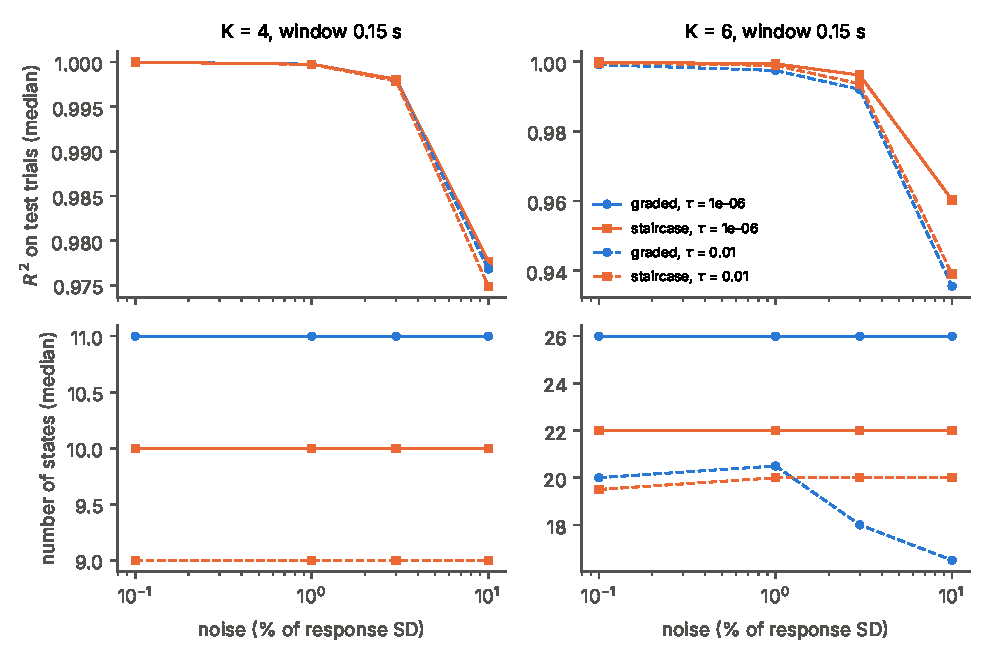
\includegraphics[width=\textwidth]{fig_regression.pdf}
\caption{$R^2$ on the test trials and number of states against noise, for the graded and staircase realisations of fitted coefficients, at two tolerances (medians over <<n_seeds>> noise draws; window 0.15\,s).}\label{fig:regression}
\end{figure}

\subsection{One starting state}
The coefficients describe the system from one starting state only, because they are Lie derivatives evaluated at $x_0$.
To show this, the coefficients of the driven oscillator fitted at $K=6$ without noise to trials that start from $x_0$ were used, unchanged, to predict trials that start from $(0.6,0.2)$.
On those trials the $R^2$ is <<r2_other_6>>, against <<r2_same_6>> on test trials that start from $x_0$.
The fit itself is accurate; a series fitted in one window does not apply to a window that starts from another state.

\section{Volterra kernels from the coefficients}\label{sec:kernels}
The series \eqref{eq:cfs} contains the Volterra kernels.
With one input, a word with $n$ input letters is fixed by the numbers of drift letters before, between and after them:
\[w=(0^{j_0},1,0^{j_1},1,\dots,1,0^{j_n}).\]
\begin{proposition}[Kernels from words]\label{prop:kernel}
For such a word,
\begin{gather*}
I_w(t)=\int_{0<s_1<\dots<s_n<t}K_w(t;s)\,u(s_1)\cdots u(s_n)\,ds,\\
K_w(t;s)=\frac{s_1^{j_0}}{j_0!}\,\frac{(s_2-s_1)^{j_1}}{j_1!}\cdots\frac{(t-s_n)^{j_n}}{j_n!} .
\end{gather*}
Summing over the words with $n$ input letters, the $n$-th order Volterra kernel of the series is defined for all input times $s_1,\dots,s_n$ in $[0,t]$ by
\[h_n(t;s_1,\dots,s_n)=\frac1{n!}\sum_wc_wK_w(t;s_{(1)},\dots,s_{(n)}),\]
where $s_{(1)}\le\dots\le s_{(n)}$ are the same times in increasing order.
It is symmetric in its arguments, and the order-$n$ part of the response is
\[\int_0^t\!\!\cdots\!\int_0^th_n(t;s_1,\dots,s_n)\,u(s_1)\cdots u(s_n)\,ds_1\cdots ds_n .\]
\end{proposition}
\begin{proof}
Each drift letter integrates once against time, and the integrals of a run of $j$ drift letters between two input times give $(\Delta s)^j/j!$.
Each input letter fixes one of the times $s_i$.
The cube $[0,t]^n$ is the union of $n!$ ordered pieces, one for each order of the times, and the symmetric kernel takes the same values on each; the factor $1/n!$ makes the integral over the whole cube equal to the integral over one piece.
\end{proof}
The kernels depend on $x_0$, because the coefficients do.

At $K=8$ the Duffing series has <<k_n0>>, <<k_n1>>, <<k_n2>> and <<k_n3>> non-zero words with 0, 1, 2 and 3 input letters, and none with 4.
For the input $u(t)=2\sin 6\pi t+0.5\sin 14\pi t$ at $t=0.1$\,s, the contribution of each order computed from its kernel, by Gauss--Legendre quadrature on the ordered region, agrees with the contribution computed from the iterated integrals to <<k_diff>> or better.
The contributions of orders 2 and 3 are <<k_c2>> and <<k_c3>>.

The kernels are checked against the system itself, and only as a whole.
A single kernel is not a response that the oscillator produces on its own, so the system offers nothing to compare it with directly; below, kernels from fitted coefficients are compared with the kernels of the exact series, not with responses of the system.
The sum of the contributions of all orders, each computed from its kernel, should reproduce the true response.
We solved \eqref{eq:duffing} to high accuracy for the same input, at 15 times between 0.01 and 0.15\,s.
The largest difference between the sum over all kernels and the true response is <<kfull_4>>, <<kfull_6>> and <<kfull_8>> for $K=4$, 6 and 8, against a largest response of <<kfull_y>> (Figure~\ref{fig:h1}).
The difference falls as $K$ grows, because it is the error of truncating the series.
Figure~\ref{fig:h2} shows the second-order kernel over the whole square of input times.
It is symmetric about the diagonal $s_1=s_2$, and has a corner along it, where the order of the two input times changes.

\begin{figure}[t]\centering
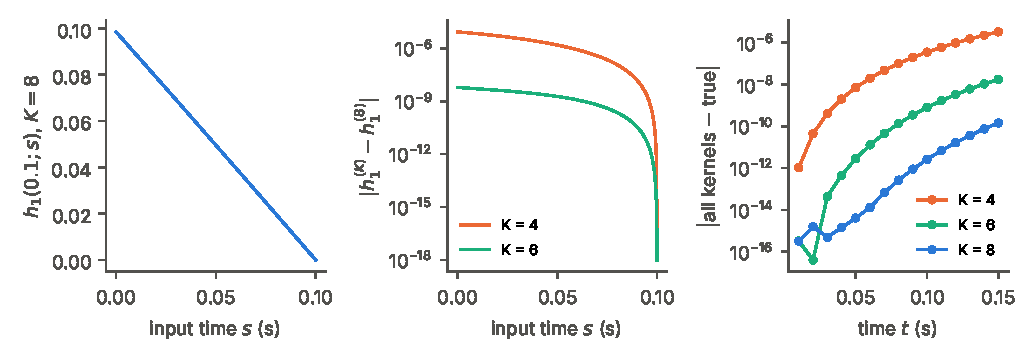
\includegraphics[width=\textwidth]{fig_h1.pdf}
\caption{Left: first-order kernel $h_1(0.1;s)$ of the series truncated at $K=8$. Middle: its difference from the kernels at $K=4$ and $K=6$. Right: difference between the response computed from all kernels of all orders and the true response of the oscillator.}\label{fig:h1}
\end{figure}
\begin{figure}[t]\centering
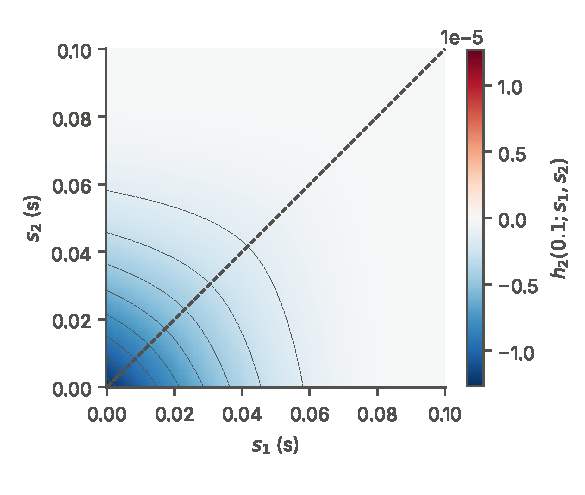
\includegraphics[width=0.55\textwidth]{fig_h2.pdf}
\caption{Symmetric second-order kernel $h_2(0.1;s_1,s_2)$ of the driven Duffing series at $K=8$, for all $s_1,s_2$ in $[0,0.1]$\,s, with contours. The dashed line is the diagonal $s_1=s_2$, about which the kernel is symmetric.}\label{fig:h2}
\end{figure}

\subsection{Kernels from fitted coefficients}
The kernels are sums of coefficients, so they inherit the imprecision of the fitted coefficients of long words.
With 1\,\% noise and the ridge penalty, the first-order kernel $h_1(0.1;s)$ of the driven oscillator has a largest error of <<h1pc_4>>\,\% of the largest value of the kernel at $K=4$ and <<h1pc_6>>\,\% at $K=6$ (medians over <<n_kdraws>> noise draws).
The second-order kernel could not be recovered.
At $K=4$ the truncated series has no second-order term at all, yet the fit gives a second-order kernel as large as <<h2e_4>>; at $K=6$ its largest error is <<h2e_6>>, against a largest value of <<h2max>>.
For the test inputs the second-order part of the series is at most <<o2part>> over 0.1-0.15\,s, far below the noise, so the data carry almost no information about it.

\subsection{Kernels without a letter for time}
Without a drift letter, every word of length $n$ has $n$ channel letters and no runs of time letters between them.
Its integral is
\[I_{(a_1,\dots,a_n)}(t)=\int_{0<s_1<\dots<s_n<t}u_{a_1}(s_1)\cdots u_{a_n}(s_n)\,ds,\]
so the order-$n$ kernel for the channels $a_1,\dots,a_n$, taken in that time order, is the constant $c_{(a_1,\dots,a_n)}$ on the ordered region.
The kernels of a path signature therefore carry no time dependence of their own: all of it comes from the inputs.
Their symmetric form, defined as in Proposition~\ref{prop:kernel} over the whole cube, is piecewise constant, with one value for each order of the channels in time.

\section{The Lyndon basis}\label{sec:lyndon}
\subsection{Lyndon words and Lie polynomials}
Many words carry overlapping information.
For example, the integrals of $(0,1)$ and $(1,0)$ in Example~\ref{ex:integrals} add up to $t\,I_{(1)}(t)$, the product of the integrals of $(0)$ and $(1)$.
Lyndon words select a set of words from which all the others can be built by such products.
They do not remove any word from a linear model: the integral of a non-Lyndon word is a polynomial in the integrals of Lyndon words, not a weighted sum of them.

Order the letters $0<1<\dots<m$, and compare words as in a dictionary.
A rotation of a word moves some of its first letters to the end; the rotations of $(0,0,1)$ are $(0,1,0)$ and $(1,0,0)$.
A word is a Lyndon word if it comes strictly before each of its rotations.
So $(0,1)$ is a Lyndon word, and $(1,0)$ and $(0,0)$ are not.
With one input, the Lyndon words up to length 4 are
\[(0),\ (1),\ (0,1),\ (0,0,1),\ (0,1,1),\ (0,0,0,1),\ (0,0,1,1),\ (0,1,1,1).\]
There are 2, 1, 2, 3, 6, 9, 18 and 30 of lengths 1 to 8, against $2^L$ words of length $L$.

Each Lyndon word $l$ of length at least 2 is split as $l=uv$, where $v$ is its longest proper ending that is itself a Lyndon word; then $u$ is a Lyndon word too \cite{ChenFoxLyndon1958}.
The standard bracketing of $l$ is the combination of words $P_l=P_uP_v-P_vP_u$, with $P_a=a$ for a single letter.
For example,
\[P_{(0,1)}=(0,1)-(1,0),\qquad P_{(0,0,1)}=(0,0,1)-2\,(0,1,0)+(1,0,0).\]
Each $P_l$ is built from commutators, and is called a Lie polynomial.
The $P_l$, for $l$ a Lyndon word, form a basis of all Lie polynomials \cite{Reutenauer1993}.

The Lie polynomials have a meaning for the system \eqref{eq:system}.
Extend the coefficients to combinations of words by linearity, so that $c_{P_{(0,1)}v}=c_{(0,1)v}-c_{(1,0)v}$.
This is the difference between applying the drift and then the input, and applying the input and then the drift.
By \eqref{eq:cfs} it equals $\bigl((L_{f_0}L_{f_1}-L_{f_1}L_{f_0})L_vh\bigr)(x_0)$.
The commutator of two Lie derivatives is the Lie derivative along a third vector field, the Lie bracket $[f_0,f_1]$, defined so that $L_{[f,g]}=L_fL_g-L_gL_f$: a direction in which the state can be moved by alternating drift and input.
In the same way, for every Lyndon word,
\begin{equation}\label{eq:liecoef}
c_{P_lv}=\bigl(L_{F_l}L_vh\bigr)(x_0),
\end{equation}
where $F_l$ is the bracket of the vector fields $f_0,\dots,f_m$ named by $P_l$.

\subsection{The Lie--Hankel matrix}
The Lie--Hankel matrix of a series has one row for each Lyndon word $l$ and one column for each word $v$, with entry $c_{P_lv}$.
The Lie--Hankel matrix of a series truncated at order $K$ uses the same convention as the staircase matrix: rows of length 1 to $K$, columns of length 0 to $K$, and entries with $|l|+|v|>K$ set to zero, because those are coefficients of the truncated series beyond order $K$.
Every row is a Lie polynomial with no constant term, so the empty-word coefficient $c_{()}$, and with it the starting value, never enters either matrix.

\begin{proposition}\label{prop:lie}
For the (untruncated) series of a system \eqref{eq:system} with $n$ states, the Lie--Hankel matrix has rank at most $n$.
\end{proposition}
\begin{proof}
By \eqref{eq:liecoef}, $c_{P_lv}=\nabla(L_vh)(x_0)\cdot F_l(x_0)$.
Each entry is the product of a row vector that depends only on $v$ and a column vector that depends only on $l$, both of length $n$.
\end{proof}
Fliess showed more \cite{Fliess1983}: a series has a realisation of the form \eqref{eq:system} with analytic vector fields, near $x_0$, if and only if the rank of its Lie--Hankel matrix (its Lie rank) is finite, under a convergence condition that every polynomial series meets; the smallest such realisation then has as many states as the Lie rank.
This is the nonlinear counterpart of the result for the ordinary Hankel matrix and bilinear systems.
Realisations of series that are polynomials, and nilpotent approximations, were studied computationally by Hoang Ngoc Minh, Jacob and Oussous \cite{HoangJacobOussous1991} and by Oussous \cite{Oussous1991a,Oussous1991b}; the existence and uniqueness of minimal nonlinear realisations go back to Sussmann \cite{Sussmann1977}.

For the full driven Duffing series the Lie rank is 2.
This follows from Proposition~\ref{prop:lie}, which bounds it by 2, and from its smallest block, rows $(0),(1)$ and columns $(),(0),(1)$, which already has rank 2; the blocks computed from exact coefficients up to length <<lie_maxlen>> confirm it.
A bilinear system is linear in its state, so a bilinear realisation needs extra states to represent the cubic term, and the ordinary Hankel rank grows with the order.

Table~\ref{tab:lie} gives the rank of the Lie--Hankel matrix of the truncated series, with its zeros beyond order $K$.
It grows with $K$, more slowly than the staircase rank.
The truncated series is a polynomial, not the series of the oscillator, and by Fliess's result its smallest nonlinear realisation needs this many states.
The staircase rank, the size of its smallest bilinear realisation, is larger at every order.
The Lie--Hankel matrix does not by itself give a bilinear realisation; its value here is to separate the number of states of a nonlinear model from the size of a bilinear approximation.

\begin{table}[t]\centering\small
\caption{Rank of the Lie--Hankel matrix of the driven Duffing series truncated at order $K$ (rows: Lyndon words up to length $K$; columns: all words up to length $K$; entries beyond order $K$ zero), and the staircase rank, the minimal bilinear size, from Table~\ref{tab:dims}.}\label{tab:lie}
<<tab_lie>>
\end{table}

The same holds without a drift.
The full driftless Duffing series has Lie rank <<dd_lie>>, its number of states, while the Lie--Hankel ranks of its truncations are <<dd_lie_trunc>> for $K=2$ to 8, against staircase ranks of <<dd_st_list>>.
For the Heisenberg integrator, whose series is finite, the Lie rank is <<hb_lie>>, its number of states, against a minimal bilinear realisation with <<hb_st>> states.

From fitted coefficients the Lie--Hankel matrix has a sharp gap in its singular values, but at the wrong place.
Its rank is <<lie_fit_4>> at $K=4$ and <<lie_fit_6>> at $K=6$, with or without noise, which is the largest possible value for any series truncated at that order (Table~\ref{tab:generic}).
The errors in the coefficients of long words fill every direction that truncation allows, so the fitted rank carries no information about the system.

\subsection{Lyndon words in the regression}
Products of iterated integrals are sums of iterated integrals: $I_uI_v$ is the sum of $I_w$ over all the ways $w$ of interleaving the letters of $u$ and $v$ while keeping the order within each \cite{Ree1958}.
For example, $I_{(0)}I_{(1)}=I_{(0,1)}+I_{(1,0)}$ and $I_{(1)}^2=2I_{(1,1)}$.
Every word $w$ can be written in one way as a sequence of Lyndon words that never increase, $w=l_1^{n_1}\cdots l_k^{n_k}$ with $l_1>\dots>l_k$ \cite{ChenFoxLyndon1958}.
The products
\[R_w=\frac{I_{l_1}^{n_1}\cdots I_{l_k}^{n_k}}{n_1!\cdots n_k!}\]
form a second basis, in which every iterated integral is a polynomial in the integrals of Lyndon words \cite{Radford1979,Reutenauer1993}.
For example, $(1,0)$ splits as $(1)(0)$, and $R_{(1,0)}=I_{(1)}I_{(0)}=I_{(0,1)}+I_{(1,0)}$.

Lyndon words have been used in two other ways for regression on iterated integrals.
One uses only the Lyndon words as regressors.
The other uses the log-signature: the logarithm of the series $\sum_wI_w\,w$, taken in the algebra of words, which is a Lie polynomial and so is fixed by one coordinate for each Lyndon word, and reads the response as a weighted sum of those coordinates.
Table~\ref{tab:lynreg} compares the four choices at $K=6$.

\begin{table}[t]\centering\small
\caption{Regression in four bases at $K=6$, 0.15\,s, all with the ridge penalty. $R^2$ on the test trials without noise and at 1\,\% noise (standard deviation 1\,\% of that of the response) (median over <<n_seeds>> draws). The Lyndon products give the same model as all words; with least squares their predictions agree to <<rad_diff>>.}\label{tab:lynreg}
<<tab_lynreg>>
\end{table}

Fitting the response to the $R_w$ instead of the $I_w$ is the same model in different coordinates, because each set is an invertible combination of the other.
On the test trials the two fits agree to within <<rad_diff>>.
The condition number is worse: <<rad_cond_6>> in the Lyndon basis, against <<cond_6>> in the word basis.
This is general: the uncertainty of any coefficient, or of any kernel, does not depend on the coordinates in which the model is written, and a change of coordinates only moves the ill-conditioning into the map between them.

The other two are different, smaller models with <<lyn_n_6>> instead of <<ncol_6>> coefficients.
Products of Lyndon integrals are not weighted sums of them; $I_{(1,1)}=\tfrac12I_{(1)}^2$ is a square, and no weighted sum of Lyndon integrals can produce it.
The same holds for the log-signature coordinates.
Both models are much better conditioned, because they have far fewer coefficients, and both lose accuracy.
With the ridge penalty in every case, their $R^2$ on the test trials stays well below that of the full series both without noise and at 1\,\% noise (Table~\ref{tab:lynreg}): their error is mainly one of the model, not of noise.
The useful role of Lyndon words is therefore the Lie--Hankel matrix of the previous section, not a basis for the fit.

\section{Practical lessons}\label{sec:lessons}
\begin{enumerate}
\item Compute iterated integrals exactly when the input is a formula, and with iisignature on the sampled path when it is data. Report which was used and the sampling error, which for long words is far larger than for short ones.
\item Build the Hankel matrix of a truncated series with rows and columns of all words up to length $K$, and zeros wherever the combined word is longer than $K$. Its rank gives the minimal realisation, which is nilpotent.
\item The graded construction stays nilpotent when it is reduced, but it is larger, and in the examples its guarantee did not change any prediction within the window.
\item Shift each window to start at zero and fit a free offset for each window.
\item Judge a fit by its $R^2$ on data not used for fitting. Use a ridge penalty chosen on separate validation data, and enough trials for the number of coefficients.
\item Compare coefficients only on the scale $c_wT^L/L!$, and only as relative errors. The coefficients of long words could not be fitted correctly from noisy data; the response could.
\item The sizes of realisations of fitted series, and their Lie--Hankel ranks, sit at the largest values possible for the order. Compare any such size with that ceiling before using it as a measure.
\item Validate kernels only through the full series: summed over all orders, they must reproduce the true response. Without a drift, the kernels are the coefficients themselves.
\item A truncated series, and so its realisation, describes the system near the starting state only: within a window of time with a drift, and without one only while the iterated integrals of the path, including the areas it sweeps, stay small. A finite series, such as that of the Heisenberg integrator, is the exception.
\item Lyndon words give the Lie--Hankel matrix, whose rank counts the states of a nonlinear model. As a basis for the fit they give the same fit or a smaller, less accurate model.
\end{enumerate}

\section*{Code availability}
The code that produces every number, table and figure of this tutorial is released with it as an open-source package under the MIT licence; its README explains how to use it.

\begin{thebibliography}{99}
\bibitem{BerstelReutenauer2011} J.~Berstel and C.~Reutenauer, Noncommutative Rational Series with Applications, Encyclopedia of Mathematics and its Applications 137, Cambridge University Press, 2011.
\bibitem{Brockett1976} R.~W.~Brockett, Volterra series and geometric control theory, Automatica 12(2):167-176, 1976.
\bibitem{Chen1957} K.-T.~Chen, Integration of paths, geometric invariants and a generalized Baker-Hausdorff formula, Annals of Mathematics 65(1):163-178, 1957.
\bibitem{ChenFoxLyndon1958} K.-T.~Chen, R.~H.~Fox and R.~C.~Lyndon, Free differential calculus IV. The quotient groups of the lower central series, Annals of Mathematics 68(1):81-95, 1958.
\bibitem{ChevyrevKormilitzin2016} I.~Chevyrev and A.~Kormilitzin, A primer on the signature method in machine learning, arXiv:1603.03788, 2016.
\bibitem{Crouch1981} P.~E.~Crouch, Dynamical realizations of finite Volterra series, SIAM Journal on Control and Optimization 19(2):177-202, 1981.
\bibitem{DAlessandroIsidoriRuberti1974} P.~d'Alessandro, A.~Isidori and A.~Ruberti, Realization and structure theory of bilinear dynamical systems, SIAM Journal on Control 12(3):517-535, 1974.
\bibitem{Fliess1974} M.~Fliess, Matrices de Hankel, Journal de Math\'ematiques Pures et Appliqu\'ees 53:197-224, 1974.
\bibitem{Fliess1981} M.~Fliess, Fonctionnelles causales non lin\'eaires et ind\'etermin\'ees non commutatives, Bulletin de la Soci\'et\'e Math\'ematique de France 109:3-40, 1981.
\bibitem{Fliess1983} M.~Fliess, R\'ealisation locale des syst\`emes non lin\'eaires, alg\`ebres de Lie filtr\'ees transitives et s\'eries g\'en\'eratrices non commutatives, Inventiones Mathematicae 71(3):521-537, 1983.
\bibitem{FrizVictoir2010} P.~K.~Friz and N.~B.~Victoir, Multidimensional Stochastic Processes as Rough Paths, Cambridge University Press, 2010.
\bibitem{HairerNorsettWanner1993} E.~Hairer, S.~P.~N{\o}rsett and G.~Wanner, Solving Ordinary Differential Equations I: Nonstiff Problems, 2nd edition, Springer, 1993.
\bibitem{HespelJacob1991} C.~Hespel and G.~Jacob, Approximation of nonlinear dynamic systems by rational series, Theoretical Computer Science 79(1):151-162, 1991.
\bibitem{HespelJacob1998} C.~Hespel and G.~Jacob, First steps towards exact algebraic identification, Discrete Mathematics 180(1-3):211-219, 1998.
\bibitem{HoangJacobOussous1991} Hoang Ngoc Minh, G.~Jacob and N.~E.~Oussous, Input/output behaviour of nonlinear analytic systems: rational approximations, nilpotent structural approximations, in B.~Bonnard, B.~Bride, J.-P.~Gauthier and I.~Kupka (eds), Analysis of Controlled Dynamical Systems, Progress in Systems and Control Theory 8, Birkh\"auser, 1991, pp.~255-262.
\bibitem{HoKalman1966} B.~L.~Ho and R.~E.~Kalman, Effective construction of linear state-variable models from input/output functions, Regelungstechnik 14:545-548, 1966.
\bibitem{Isidori1973} A.~Isidori, Direct construction of minimal bilinear realizations from nonlinear input-output maps, IEEE Transactions on Automatic Control 18(6):626-631, 1973.
\bibitem{Isidori1995} A.~Isidori, Nonlinear Control Systems, 3rd edition, Springer, 1995.
\bibitem{Kalman1963} R.~E.~Kalman, Mathematical description of linear dynamical systems, SIAM Journal on Control 1:152-192, 1963.
\bibitem{Krener1975} A.~J.~Krener, Bilinear and nonlinear realizations of input-output maps, SIAM Journal on Control 13(4):827-834, 1975.
\bibitem{Lyons1998} T.~J.~Lyons, Differential equations driven by rough signals, Revista Matem\'atica Iberoamericana 14(2):215-310, 1998.
\bibitem{Oussous1991a} N.~E.~Oussous, Computation, on Macsyma, of the minimal differential representation of noncommutative polynomials, Theoretical Computer Science 79(1):195-207, 1991.
\bibitem{Oussous1991b} N.~E.~Oussous, Macsyma computation of local minimal realization of dynamical systems of which generating power series are finite, Journal of Symbolic Computation 12:115-126, 1991.
\bibitem{Radford1979} D.~E.~Radford, A natural ring basis for the shuffle algebra and an application to group schemes, Journal of Algebra 58(2):432-454, 1979.
\bibitem{Ree1958} R.~Ree, Lie elements and an algebra associated with shuffles, Annals of Mathematics 68(2):210-220, 1958.
\bibitem{ReizensteinGraham2020} J.~F.~Reizenstein and B.~Graham, Algorithm 1004: the iisignature library: efficient calculation of iterated-integral signatures and log signatures, ACM Transactions on Mathematical Software 46(1):8, 2020.
\bibitem{Reutenauer1993} C.~Reutenauer, Free Lie Algebras, London Mathematical Society Monographs 7, Oxford University Press, 1993.
\bibitem{Schutzenberger1961} M.~P.~Sch\"utzenberger, On the definition of a family of automata, Information and Control 4:245-270, 1961.
\bibitem{Shaikin2004} M.~E.~Shaikin, Optimal estimation equations for state vector of a stochastic bilinear system: its bilinear approximation, Automation and Remote Control 65(12):1946-1960, 2004.
\bibitem{Sontag1979} E.~D.~Sontag, Polynomial Response Maps, Lecture Notes in Control and Information Sciences 13, Springer, 1979.
\bibitem{Sussmann1977} H.~J.~Sussmann, Existence and uniqueness of minimal realizations of nonlinear systems, Mathematical Systems Theory 10:263-284, 1977.
\bibitem{Volterra1930} V.~Volterra, Theory of Functionals and of Integral and Integro-Differential Equations, Blackie, 1930.
\bibitem{WrayGreen1994} J.~Wray and G.~G.~R.~Green, Calculation of the Volterra kernels of non-linear dynamic systems using an artificial neural network, Biological Cybernetics 71(3):187-195, 1994.
\end{thebibliography}
\end{document}
